\documentclass[UTF8]{ctexart}
\usepackage{subfigure}
\usepackage{caption}
\usepackage{amsmath,bm}
\usepackage{amssymb}
\usepackage{pifont}
\usepackage{geometry}
\usepackage{graphicx}
\usepackage{gensymb}
\usepackage{wrapfig}
\usepackage{titlesec}
\usepackage{float}
\usepackage{diagbox}
\usepackage{fancyhdr}
\usepackage{color}
\usepackage{bm}
\usepackage{siunitx}
\usepackage{ulem}
\usepackage{CJKulem}
\pagestyle{plain}
\geometry{a4paper,scale=0.8}
\CTEXsetup[format+={\raggedright}]{section} 
\title{固物2012期中}
\author{Deschain}
\titlespacing*{\section}
{0pt}{0pt}{0pt}
\titlespacing*{\subsection}
{0pt}{0pt}{0pt}
\titlespacing*{\paragraph}
{0pt}{0pt}{0pt}
\titlespacing*{\subparagraph}
{0pt}{0pt}{0pt}
\titleformat*{\section}{\normalsize}
\begin{document}
\maketitle
\section*{\bfseries 一、填空(共20分,每空1分)}
1.金刚石晶体是\uline{\makebox[3em]{}}格子,由两个\uline{\makebox[6em]{}}结构的子晶格沿空间对角线
方向位移$\frac{1}{4}$的长度套构而成。\\
2.体心立方结构的单胞边长为$a$,那么原胞的体积为\uline{\makebox[3em]{}},对应的第一布里渊区体积为
\uline{\makebox[4em]{}}。\\
3.对于固体的能带,简约波矢$\bm{k}$的取值范围要求在\uline{\makebox[9em]{}}区域内,其取值总数等于
\uline{\makebox[3em]{}}的总数。\\
4.一般固体的结合可以概括为\uline{\makebox[6em]{}}、\uline{\makebox[6em]{}}、\uline{\makebox[7em]{}}
和\uline{\makebox[10em]{}}四种基本形式。\\
5.空穴是一种虚拟粒子,实际代表了\uline{\makebox[12em]{}}电子的总体运动。\\
6.如果一些能量区域中,波动方程不存在具有布洛赫函数形式的解,这些能量区域称为\uline{\makebox[3em]{}};
写出至少两种根据近自由电子近似理论的能带图景:\uline{\makebox[12em]{}}和\uline{\makebox[12em]{}}。
7.电子在三维周期性晶格中波函数方程的解具有\uline{\makebox[12em]{}}的形式,式中\uline{\makebox[4em]{}}
在晶格平移下保持不变(具有平移对称),其物理意义是:\uline{\makebox[25em]{}}。\\
8.能带顶部电子的有效质量为\uline{\makebox[2em]{}}(填写“正”或“负”);能带底部电子的有效质量为
\uline{\makebox[2em]{}}(填写“正”或“负”)。\\
9.电子波包的准动量$\bm{k}$与原胞边长$a$满足\uline{\makebox[10em]{}}的条件下,电子可以视为经典粒子。\\
\section*{\bfseries 二、简答题(共20分)}
1.(8分)波矢空间与倒格空间有何关系?为什么说波矢空间内的状态点是准连续的?\\
2.(6分)解释什么是有效质量?\\
3.(6分)解释什么是费米面、费米能、费米动量?\\
\section*{\bfseries 三、计算题(共60分)}
1.(15分)对面心立方布拉菲格子:\\
a.根据格点密度的大小,对$\{100\}$、$\{111\}$、$\{110\}$三个晶面按从大到小顺序进行排列。\\
b.画出这些格点在平面上格点的排布。\\
c.设惯用晶胞的边长为a,分别求出这三个晶面系相邻晶面的间距。\\
2.(15分)设两原子的相互作用能可表示为$U(r)=-\frac{\alpha}{r^2}+\frac{\beta}{r^8}$,其中$r$是两原子间距离,
$\alpha$,$\beta$是两个待定系数。当两原子构成一稳定分子时,其核间距为$3\times10^{-10}m$,离解能为$4eV$,试计算:\\
a.求$\alpha$,$\beta$的数值。
b.计算使该分子分裂所必须的力。(即该力不能小于合力表现为引力的最大值)
3.设一维晶体的电子能带可以写成$E(k)=\frac{\hbar^2}{ma^2}(\frac{9}{10}-cos(ka)+\frac{1}{10}cos(2ka))$,式中$a$
为晶格常数。试计算:\\
a.能带的宽度。\\
b.电子在波矢$k$状态时速度。\\
c.能带底部和能带顶部电子的有效质量。\\
4.(15分)具有简单立方晶格的二维金属,晶格常数为$a$,共有$N$个原胞,每个原子贡献一个价电子。\\
a.请按照自由电子气模型计算二维电子气能量标度下的态密度。\\
b.计算该金属在绝对零度下的费米半径。\\





\newpage
\section*{\bfseries 一、填空题答案}
1.\ding{172}复式\makebox[2em]{}
\ding{173}面心立方\\
2.\ding{172}$\frac{a^3}{2}$\makebox[2em]{}
\ding{173}$\frac{16\pi^3}{a^3}$\\
3.\ding{172}第一布里渊区\makebox[2em]{}
\ding{173}原胞\\
4.\ding{172}共价结合\makebox[2em]{}
\ding{173}离子结合\makebox[2em]{}
\ding{174}金属性结合\makebox[2em]{}
\ding{175}范德瓦尔斯结合\\
5.价带中其他所有的\\
6.\ding{172}禁带(带隙)\makebox[2em]{}
\ding{173}简约布里渊区图景\makebox[2em]{}
\ding{174}周期布里渊区图景\makebox[2em]{}
\ding{175}扩展布里渊区图景\\
7.\ding{172}$\Psi_{\vec k}(\vec r+\vec R_n)=e^{i\vec k\cdot\vec R_n}u_{\vec k}(\vec r)$\makebox[2em]{}
\ding{173}$u_{\vec k}(\vec r)$\makebox[2em]{}
\ding{174}Bloch电子波函数是受晶格周期调制的平面波\\
8.\ding{172}负\makebox[2em]{}
\ding{173}正\\
9.$\Delta k<<\frac{2\pi}{a}$\\
\section*{\bfseries 二、简答题答案}
1.\ding{172}波矢空间和倒格空间处于同一空间。倒格空间的基矢分别为$\bm{b_1},\bm{b_2},\bm{b_3}$,而波矢空间的基矢分别为
$\bm{\frac{b_1}{N_1}},\bm{\frac{b_2}{N_2}},\bm{\frac{b_3}{N_3}}$,$\bm{N_1}$、$\bm{N_2}$、$\bm{N_3}$
分别为沿正格子基矢方向晶体的原胞数目。(或波矢空间比倒格空间更密)\\
\ding{173}倒格空间中一个倒格点对应的体积为$\bm{b_1}\cdot(\bm{b_2}\times\bm{b_3})=\Omega^*$,波矢空间中一个波矢点
对应的体积为$\bm{\frac{b_1}{N_1}}\cdot(\bm{\frac{b_2}{N_2}}\times\bm{\frac{b_3}{N_3}})=\bm{\Omega^*}$。即波矢空间中
一个波矢点对应的体积,是倒格空间中一个倒格点对应的体积的$\bm{\frac{1}{N}}$。由于$\bm{N}$是晶体的原胞数目,数目巨大,所以
一个波矢点对应的体积与一个倒格点对应的体积相比是极其微小的。也就是说,波矢点在倒格空间看是极其稠密的。因此,在波矢空间内
作求和处理时,可把波矢空间内的状态点看成是准连续的。\\
2.晶体中的电子(或空穴)除了受到外场作用外,还要受到晶体中原子的周期势场和其他电子的平均势场的作用。在讨论
电子受外场力作用下运动时,有效质量即是把内场力等价电子部分质量的结果,其表达式为$\frac{1}{m_\alpha^*}=\frac{1}{\hbar^2}
\cdot\frac{\partial^2E}{\partial{k_\alpha}^2}$。\\
3.费米面是$\bm{k}$空间占有电子和不占有电子区域的分界面;费米面的能量是费米能;费米速度为费米面上电子所对应的速度。\\
\section*{\bfseries 三、计算题答案}
1.a.$\{111\},\{100\},\{111\}$\\
b.
\begin{figure}[H]
    \centering
    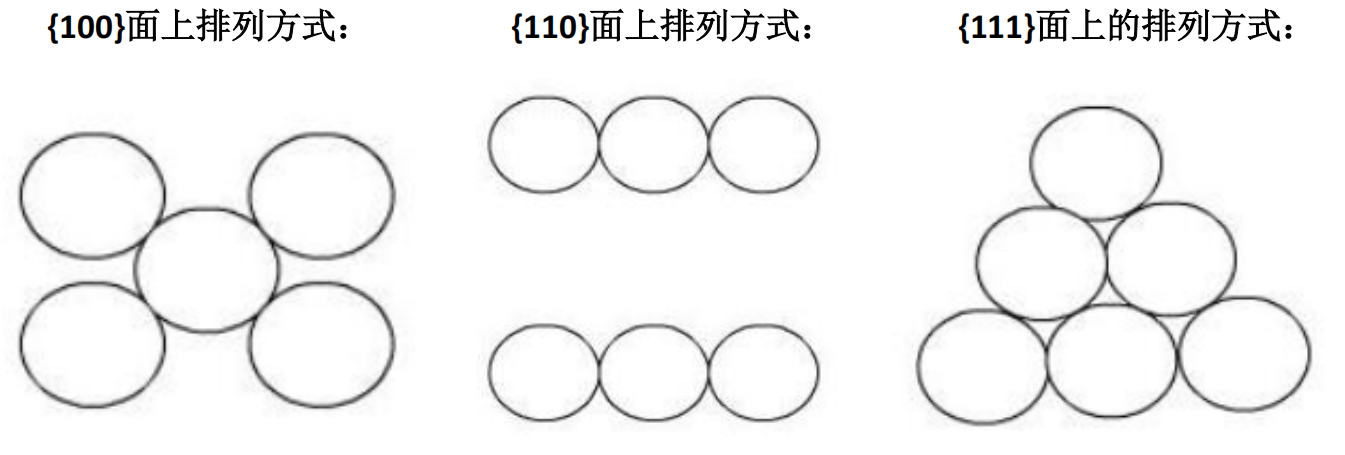
\includegraphics[width=9cm,height=4cm]{3_1_b.png}
\end{figure}
c.$\{111\}:\frac{\sqrt3}{3}a,\{100\}:\frac{1}{2}a,\{111\}:\frac{\sqrt2}{4}$\\
2.a.
\begin{equation*}
    \begin{aligned}
        & \frac{dU(r)}{dr}\Bigg\lvert_{r=r_0}=\frac{2\alpha}{r_0^3}-\frac{8\beta}{r_0^9}=0,\quad 
        r_0=(\frac{4\beta}{\alpha})^\frac{1}{6}=3\times10^{-10}m\\
        & U(r_0)=-\frac{\alpha}{r_0^2}+\frac{\beta}{r_0^8}=-\frac{3\alpha}{4r_0^2}=4eV\\
        & \alpha=7.68\times10^{-38}J\cdot m^{-2},\quad\beta=1.4\times10^{-95}J\cdot m^{-8}\\
    \end{aligned}
\end{equation*}
b.
\begin{equation*}
    \begin{aligned}
        &\frac{d^2U(r)}{dr^2}\Bigg\lvert_{r=r_m}=-\frac{6\alpha}{r_0^4}+\frac{72\beta}{r_0^10}=0,\quad
        r_m=(\frac{12\beta}{\alpha})^\frac{1}{6}=3.6\times10^{-10}\\
        &F=-\frac{\partial U(r)}{\partial r}\Bigg\lvert_{r=r_m}=-\frac{2\alpha}{r_m^3}+\frac{8\beta}{r_m^9}
        =0.22\times10^{-8}\\
    \end{aligned}
\end{equation*}
3.
a.能带底部$k=0,E(0)=0$;能带顶部$k=\frac{\pi}{a},E(\frac{\pi}{a})=\frac{2\hbar^2}{ma^2}$,能带宽度$\Delta E=
E(\frac{\pi}{a})=\frac{2\hbar^2}{ma^2}$\\
b.
\begin{equation*}
    \begin{aligned}
        & v(k)=\frac{1}{\hbar}\cdot\frac{dE(k)}{dk}=\frac{\hbar}{ma}(sin(ka)-\frac{1}{5}sin(2ka))\\
    \end{aligned}
\end{equation*}
c.
\begin{equation*}
    \begin{aligned}
        & m^*=\frac{\hbar^2}{\frac{\partial^2E}{\partial k^2}}=\frac{m}{cos(ka)-\frac{2}{5}cos(2ka)}\\
        & m^*(0)=\frac{5m}{3},\quad m^*(\frac{\pi}{a})=\frac{-5}{7}m\\
    \end{aligned}
\end{equation*}
4.
a.
\begin{equation*}
    \begin{aligned}
        & Z=2\cdot\frac{S}{4\pi^2}\cdot k^2=2\cdot\frac{Na^2}{4\pi^2}\cdot\frac{2mE}{\hbar^2}
        =\frac{mNa^2}{\pi\hbar^2}E\\
        & g(E)=\frac{dZ}{dE}=\frac{mNa^2}{\pi\hbar^2}\\
    \end{aligned}
\end{equation*}
b.
\begin{equation*}
    \begin{aligned}
        &N=\int_0^{E_F}g(E)dE,\quad E_F=\frac{\pi^2\hbar^2}{a^2m}\\
        &k_F=\sqrt{\frac{2mE}{\hbar^2}}=\sqrt{\frac{2\pi}{a^2}}=\frac{2.51}{a}\\
    \end{aligned}
\end{equation*}










\end{document}